\chapter{Implementation}

\section{Captures d'écran de l'application}

\begin{figure}[h]
    \centering
    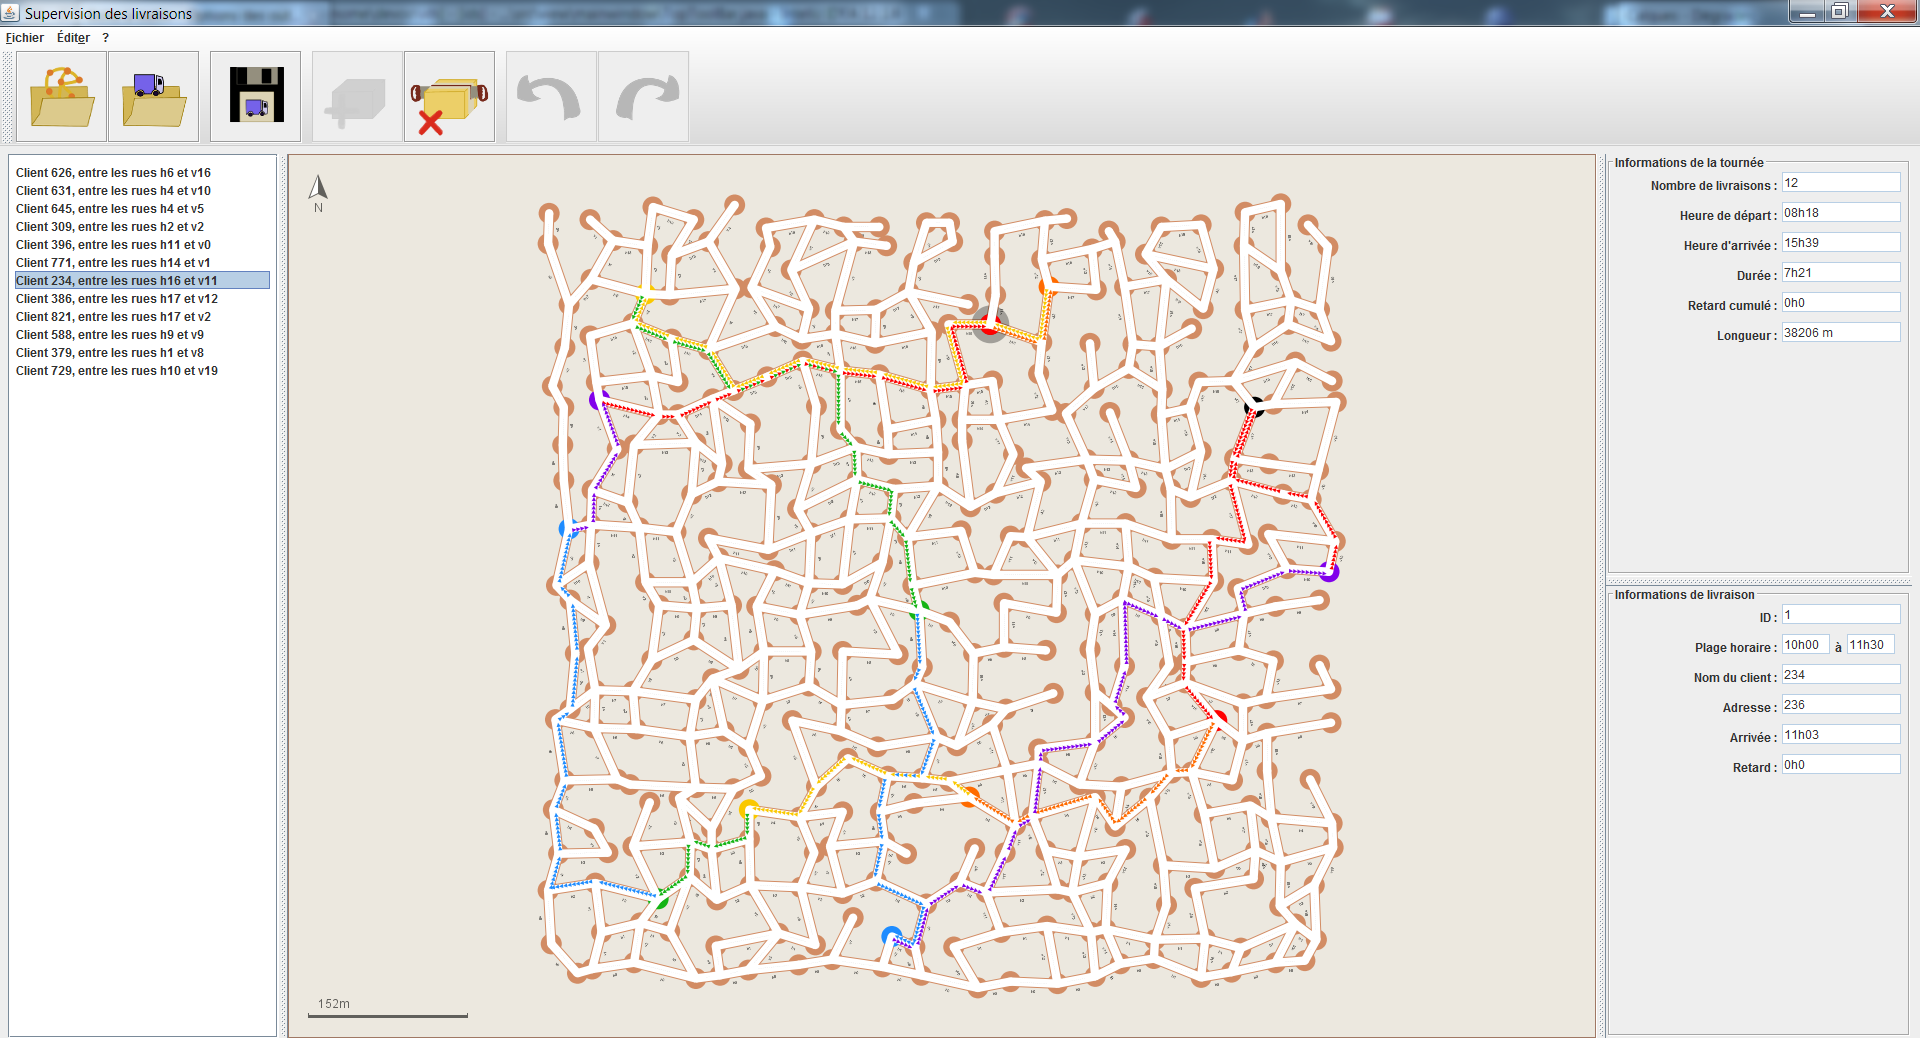
\includegraphics[width=\linewidth]{./images/screenshot1.png}
    \caption{Capture d'écran de la fenêtre principale}
\end{figure}
\pagebreak

\begin{figure}[h]
    \centering
    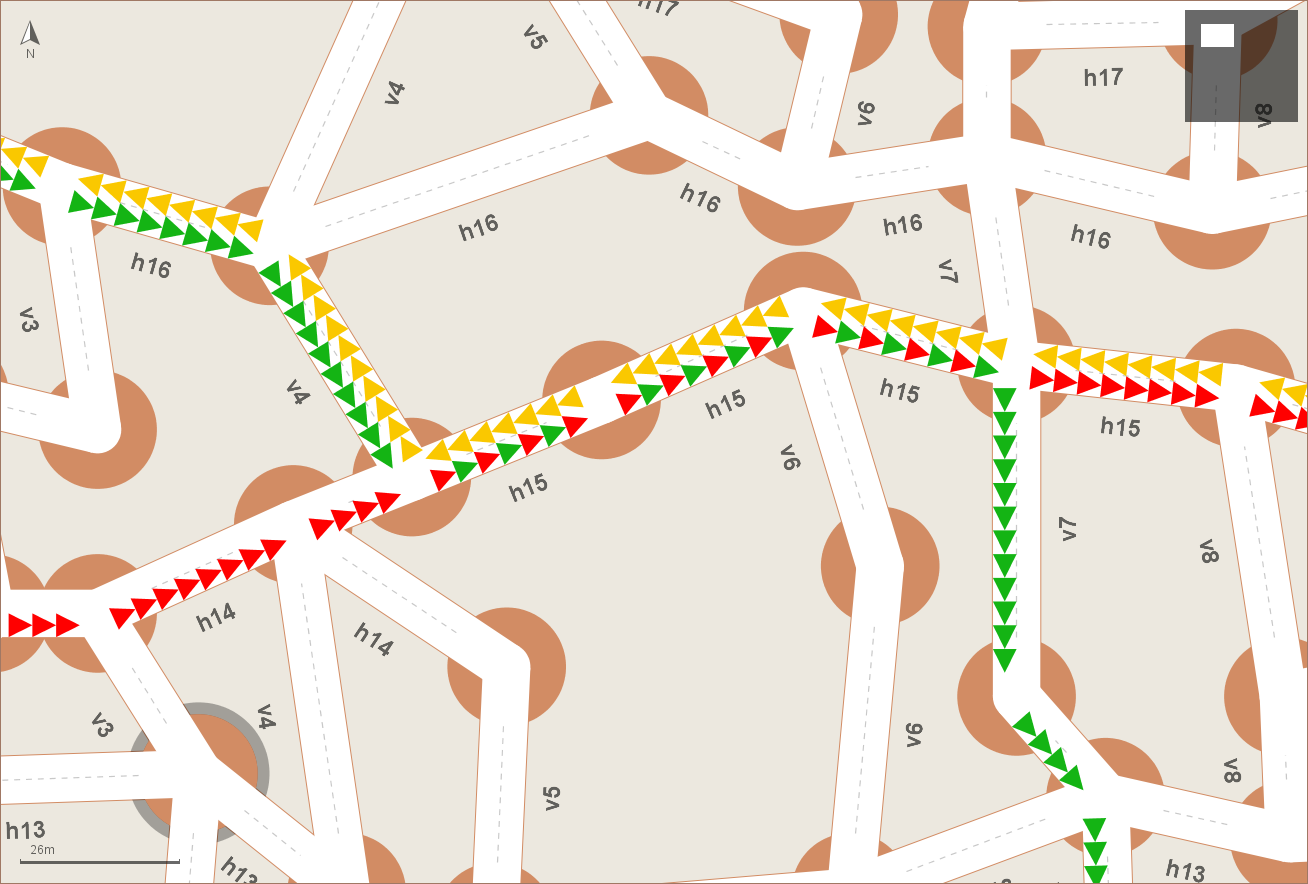
\includegraphics[width=\linewidth]{./images/screenshot2.png}
    \caption{Zoom sur le graphe}
\end{figure}
\pagebreak

\begin{figure}[h]
    \centering
    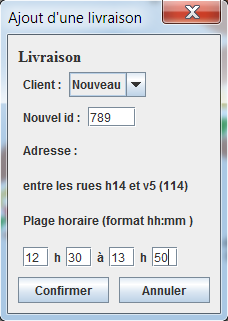
\includegraphics[width=80mm]{./images/screenshot3.png}
    \caption{Fenêtre d'ajout d'une livraison}
\end{figure}
\pagebreak

% ----------------------------------------------------------------------------- Diagrames-UML

\section{Diagrammes r\'etrog\'en\'er\'es de packages et de classes}

\subsection{Architecture g\'en\'erale de l'application}

\begin{figure}[h]
    \centering
    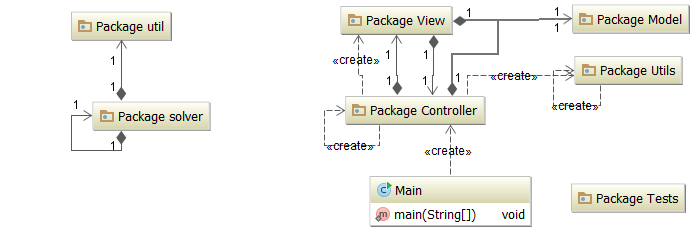
\includegraphics[width=150mm]{../diagrams/classes_packages/final_classes_packages/packages.png}
    \caption{Diagramme r\'etrog\'en\'er\'e UML de package principale}
    \label{diagram:gen_uml_global}
\end{figure}
\pagebreak

\subsection{Package Utilitaires (Utils)}

\begin{figure}[h]
    \centering
    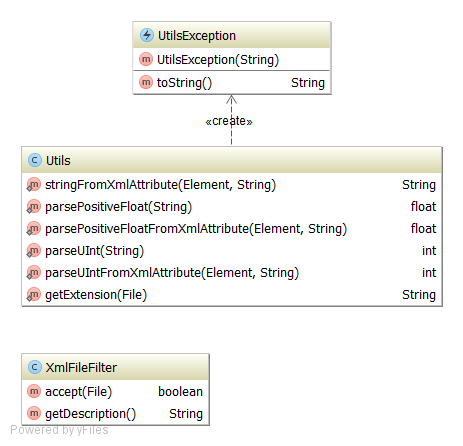
\includegraphics[width=100mm]{../diagrams/classes_packages/final_classes_packages/utils/package_utils.png}
    \caption{Diagramme r\'etrog\'en\'er\'e UML du package Utils}
    \label{diagram:gen_uml_utils}
\end{figure}
\pagebreak

\subsection{Package Mod\`ele (Model)}

\begin{figure}[h]
    \centering
    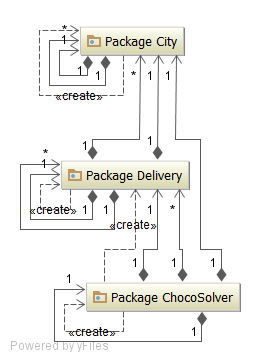
\includegraphics[width=80mm]{../diagrams/classes_packages/final_classes_packages/model/package_model.png}
    \caption{Diagramme r\'etrog\'en\'er\'e UML du package Model}
    \label{diagram:gen_uml_model}
\end{figure}
\pagebreak

\subsubsection{Package Mod\`ele.Ville (Model.City)}

\begin{figure}[h]
    \centering
    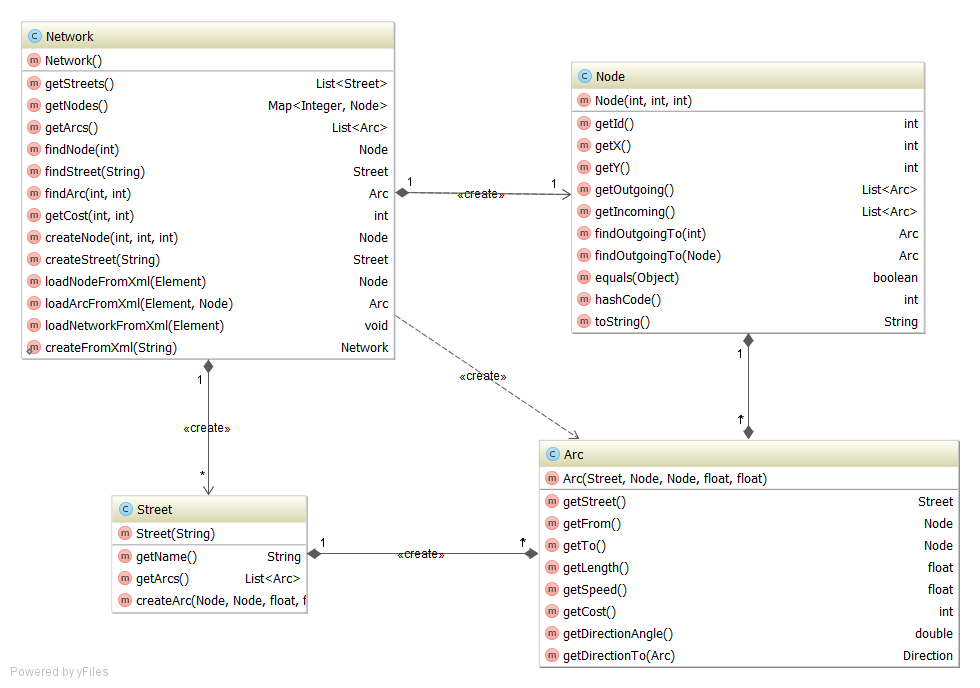
\includegraphics[width=160mm]{../diagrams/classes_packages/final_classes_packages/model/city.png}
    \caption{Diagramme r\'etrog\'en\'er\'e UML du package Model.City}
    \label{diagram:gen_uml_model_city}
\end{figure}
\pagebreak

\subsubsection{Package Mod\`ele.Livraison (Model.Delivery)}

\begin{figure}[h]
    \centering
    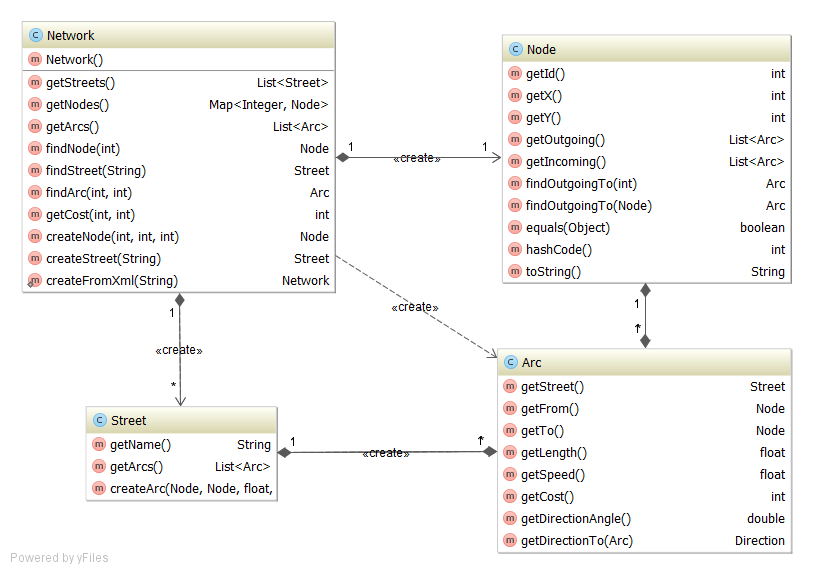
\includegraphics[width=160mm]{../diagrams/classes_packages/final_classes_packages/model/delivery.png}
    \caption{Diagramme r\'etrog\'en\'er\'e UML du package Model.Delivery}
    \label{diagram:gen_uml_model_delivery}
\end{figure}
\pagebreak

\begin{landscape}
\subsubsection{Package Mod\`ele.ChocoSolver (Model.ChocoSolver)}

\begin{figure}[h]
    \centering
    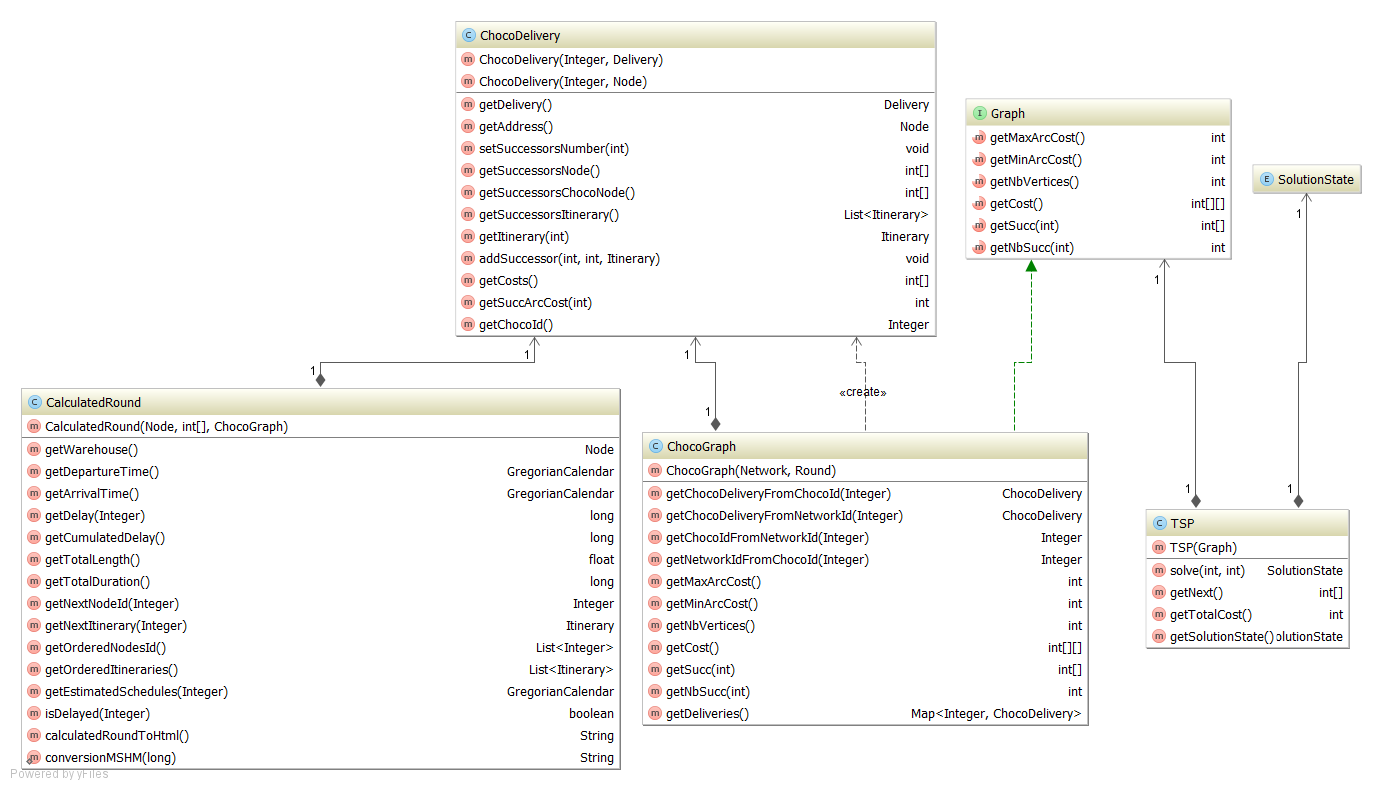
\includegraphics[width=200mm]{../diagrams/classes_packages/final_classes_packages/model/chocoSolver.png}
    \caption{Diagramme r\'etrog\'en\'er\'e UML du package Model.ChocoSolver}
    \label{diagram:gen_uml_model_choco}
\end{figure}
\end{landscape}
\pagebreak

\subsection{Package Vue (View)}

\begin{figure}[h]
    \centering
    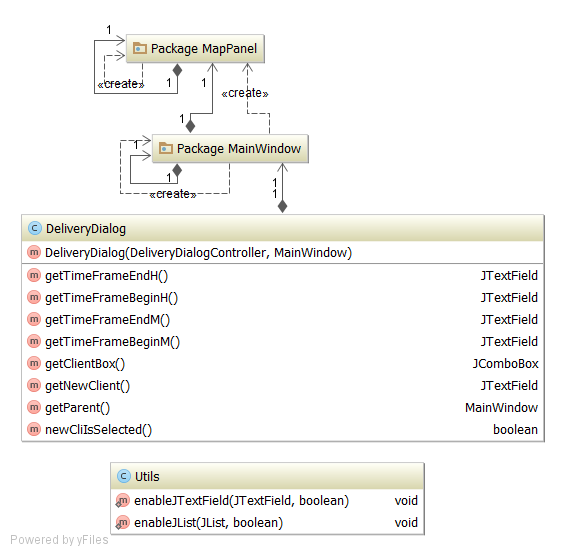
\includegraphics[width=120mm]{../diagrams/classes_packages/final_classes_packages/view/view.png}
    \caption{Diagramme r\'etrog\'en\'er\'e UML du package View}
    \label{diagram:gen_uml_view}
\end{figure}
\pagebreak

\subsubsection{Package Vue.Carte (View.MapPanel)}

\begin{figure}[h]
    \centering
    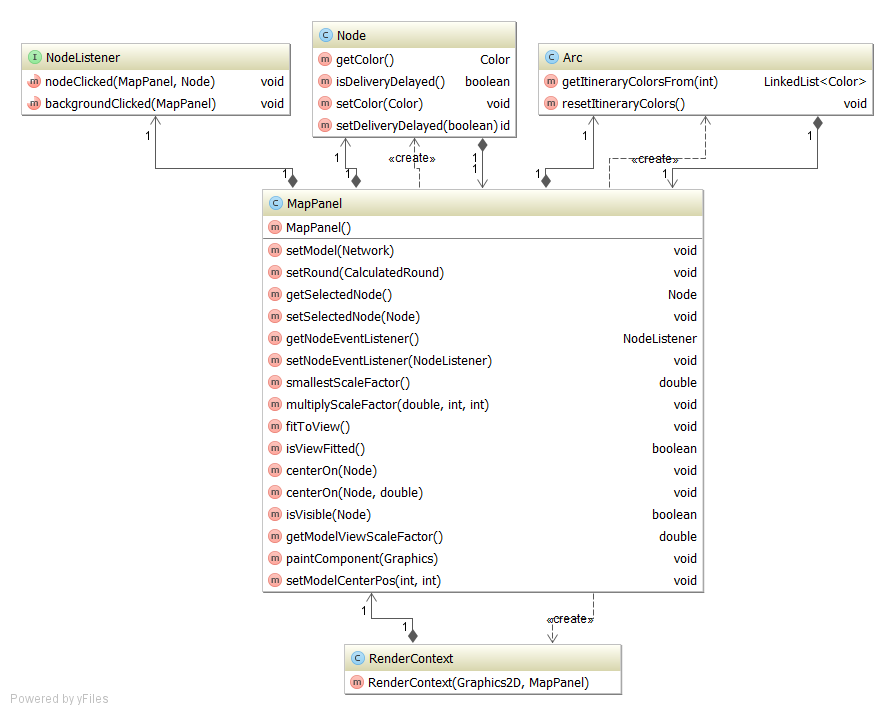
\includegraphics[width=160mm]{../diagrams/classes_packages/final_classes_packages/view/package_map.png}
    \caption{Diagramme r\'etrog\'en\'er\'e UML du package View.MapPanel}
    \label{diagram:gen_uml_view_map}
\end{figure}
\pagebreak

\subsection{Package Controlleur (Controller)}

\begin{figure}[h]
    \centering
    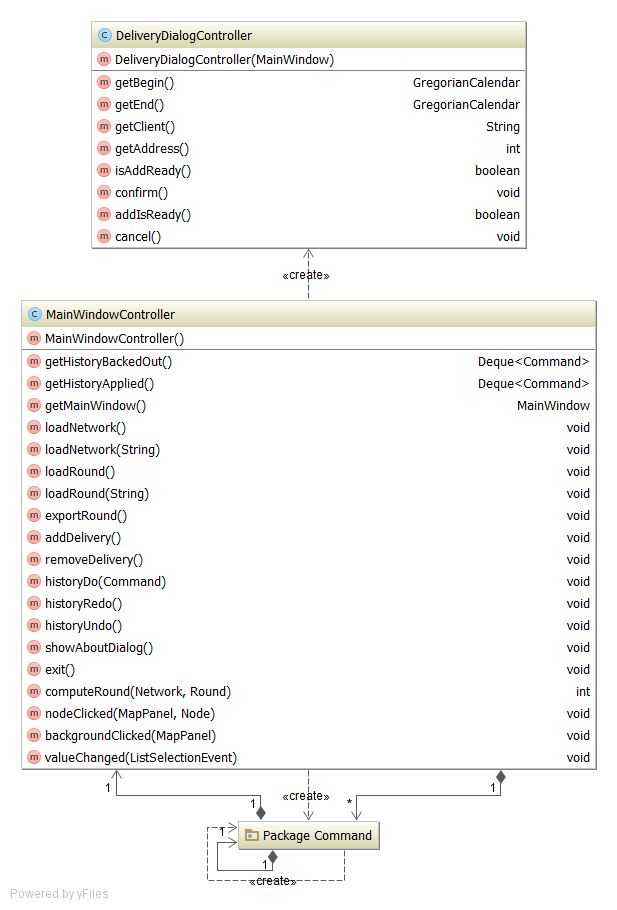
\includegraphics[width=100mm]{../diagrams/classes_packages/final_classes_packages/controller/controller.png}
    \caption{Diagramme r\'etrog\'en\'er\'e UML du package Controller}
    \label{diagram:gen_uml_controller}
\end{figure}
\pagebreak

\begin{landscape}
\subsubsection{Package Controlleur.Commande (Controller.Command)}

\begin{figure}[h]
    \centering
    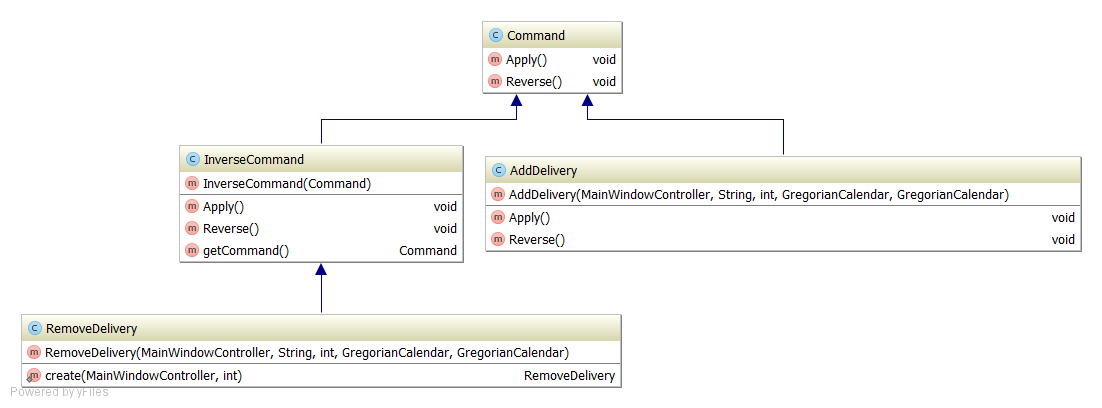
\includegraphics[width=240mm]{../diagrams/classes_packages/final_classes_packages/controller/package_command.png}
    \caption{Diagramme r\'etrog\'en\'er\'e UML du package Controller.Command}
    \label{diagram:gen_uml_controller_command}
\end{figure}
\end{landscape}

